\documentclass{article}
\usepackage[utf8]{inputenc}
\usepackage{graphicx}

\title{Problem 1}
\author{Jil Mehta (40089806) }

\begin{document}

\maketitle

\section{Introduction}
The Gaussian integral is  also known as the \textbf{Euler–Poisson integral}. It is the integral of the Gaussian function  \begin{equation} e^{-x^2} \end{equation} over the entire real line. It is named after the German mathematician Carl Friedrich Gauss.
\item
The integral can be represented as : 
\begin{figure}[htp]
    \centering
    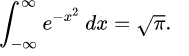
\includegraphics [width=2cm]{img}
\end{figure}

\section{Uses}
\begin{itemize}
    \item 
    Mainly used in the field of advanced Mathematics and physics (eg. quantum field theory)
\item
They are used to find indefinite integrals of any function in Mathematics.
\item
Required for evaluating the constant for the Normal Distribution.
\end{itemize}

\section{Characteristics}
\begin{itemize}
\item 
The graph for the function whose indefinite integral is to calculated is a normal distribution curve.
\item
Aims at finding the volume under the curve of the function
\item
The Gaussian Integral can be computed using 2 well known methods:
\item[]i) By Polar Coordinates
\item[]ii) By Cartesian Coordinates
\item
The integrand is always an even function.
\end{itemize}


\end{document}
